\section{AI Lấy Dữ liệu làm Trung tâm (Data-centric AI)}
\label{sec:data_centric_ai}

\subsection{Sự Chuyển dịch Mô thức: Từ Model-centric sang Data-centric}
\label{subsec:paradigm_shift_model_to_data}
Trong suốt thập kỷ đầu tiên của cuộc cách mạng học sâu (khoảng 2012-2020), sự chú ý của cộng đồng nghiên cứu và kỹ thuật gần như hoàn toàn tập trung vào mô hình. Cuộc chạy đua của \textbf{AI Lấy Mô hình làm Trung tâm (Model-centric AI)} đã tạo ra những bước nhảy vọt đáng kinh ngạc:
\begin{itemize}
	\item Các kiến trúc ngày càng sâu và phức tạp hơn, từ AlexNet, VGG, ResNet đến Transformer.
	\item Các thuật toán tối ưu hóa mới, các hàm kích hoạt hiệu quả hơn, và các kỹ thuật chính quy hóa tinh vi.
	\item Các cuộc thi benchmark như ImageNet trở thành đấu trường để so tài về thiết kế kiến trúc, nơi những cải tiến về tỷ lệ lỗi, dù chỉ là một phần trăm, cũng được xem là thành công lớn.
\end{itemize}
Trong mô thức này, bộ dữ liệu thường được coi là một hằng số, một thực thể tĩnh. Các nhóm nghiên cứu sẽ tải về một bộ dữ liệu chuẩn, đóng băng nó, và sau đó lặp đi lặp lại việc tinh chỉnh mô hình để tối đa hóa hiệu năng.

Tuy nhiên, khi các kiến trúc bắt đầu tiệm cận sự bão hòa về hiệu năng và AI bắt đầu được triển khai rộng rãi vào các ứng dụng trong thế giới thực, một sự thật quan trọng đã dần lộ rõ:
\begin{center}
	\textit{"Hiệu năng của một hệ thống AI trong thực tế không còn bị giới hạn bởi mô hình, mà bị giới hạn bởi chất lượng của dữ liệu mà nó học từ đó."}
\end{center}
Sự nhận thức này đã khai sinh ra một triết lý mới, được tiên phong và phổ biến bởi Andrew Ng: \textbf{AI Lấy Dữ liệu làm Trung tâm (Data-centric AI)}. Triết lý này đề xuất một sự đảo ngược trong tư duy: thay vì giữ nguyên dữ liệu và tinh chỉnh mô hình, hãy \textbf{giữ nguyên (hoặc thay đổi ít) mô hình và tập trung vào việc cải thiện một cách có hệ thống chất lượng của dữ liệu.}

\subsection{Các Nguyên tắc Cốt lõi của Data-centric AI}
\label{subsec:data_centric_principles}
Data-centric AI không phải là một thuật toán, mà là một tập hợp các nguyên tắc và một quy trình làm việc có hệ thống, xem dữ liệu không phải là "nguyên liệu thô" mà là "mã nguồn" của hệ thống AI.

\begin{description}
	\item[Chất lượng hơn Số lượng:] Một bộ dữ liệu nhỏ hơn nhưng có nhãn sạch, nhất quán và bao phủ tốt các trường hợp quan trọng thường mang lại kết quả tốt hơn một bộ dữ liệu lớn gấp nhiều lần nhưng đầy nhiễu và lỗi gán nhãn.
	\item[Tính Nhất quán (Consistency):] Nhãn phải nhất quán. Nếu hai người gán nhãn (annotators) nhìn vào cùng một ảnh và đưa ra các quyết định khác nhau, đó là một tín hiệu nhiễu cho mô hình. Việc thiết lập các hướng dẫn gán nhãn rõ ràng và đo lường sự đồng thuận giữa các annotator là tối quan trọng.
	\item[Độ bao phủ và Đa dạng (Coverage and Diversity):] Dữ liệu phải phản ánh được sự đa dạng của thế giới thực. Một mô hình nhận dạng xe hơi chỉ được huấn luyện trên ảnh xe sedan chạy ban ngày sẽ thất bại thảm hại khi gặp một chiếc xe tải vào ban đêm hoặc một chiếc xe thể thao bị che khuất một phần. Việc xác định và bổ sung các "trường hợp rìa" (edge cases) là một phần cốt lõi của quy trình.
	\item[Giảm thiểu Thiên vị và Tăng cường Công bằng (Bias and Fairness):] Dữ liệu trong thế giới thực thường chứa đựng các thiên vị (biases) của xã hội. Nếu một bộ dữ liệu nhận dạng khuôn mặt chứa chủ yếu là người da trắng, mô hình sẽ hoạt động kém trên các chủng tộc khác. Data-centric AI đặt việc kiểm tra, đo lường và giảm thiểu thiên vị trong dữ liệu làm ưu tiên hàng đầu.
\end{description}

\subsection{Quy trình Data-centric cho Thị giác Máy tính}
\label{subsec:data_centric_workflow}
Áp dụng triết lý Data-centric vào một dự án thị giác máy tính bao gồm một vòng lặp liên tục, thay vì một quy trình tuyến tính.

\begin{center}
	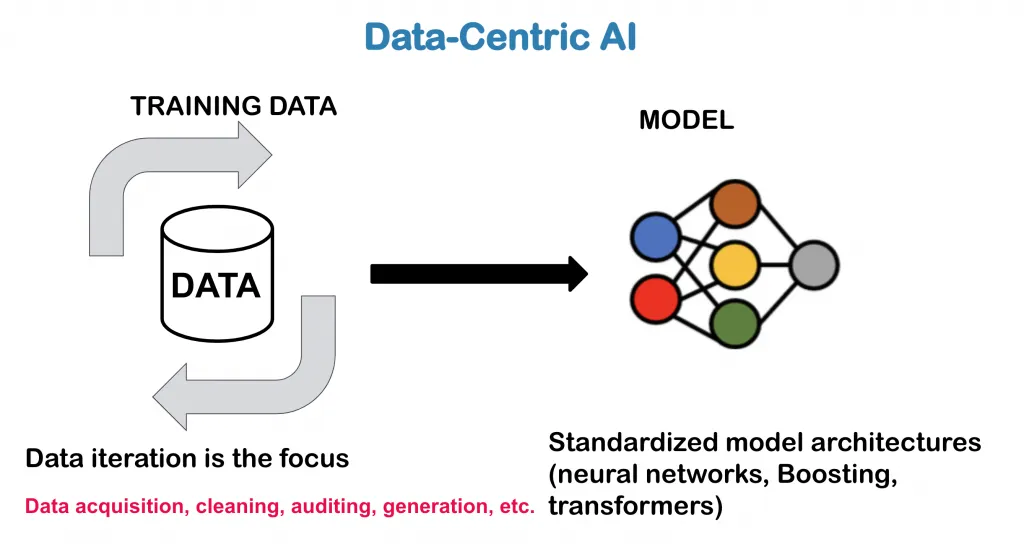
\includegraphics[width=0.9\textwidth]{images/data_centric_ai_loop.png}
	\captionof{figure}{Vòng lặp của AI Lấy Dữ liệu làm Trung tâm. Thay vì là một quy trình một chiều, nó là một chu trình liên tục: huấn luyện mô hình, phân tích lỗi, cải thiện dữ liệu, và lặp lại.}
	\label{fig:data_centric_loop}
\end{center}
% Keyword gợi ý: data-centric ai loop, data-centric ai workflow

\begin{enumerate}
	\item \textbf{Bước 1: Kiểm toán và Khám phá Dữ liệu (Data Audit):}
	Sử dụng các công cụ trực quan hóa dữ liệu (như \textbf{FiftyOne}, \textbf{Weights \& Biases}) để "nhìn" vào bộ dữ liệu của bạn.
	\begin{itemize}
		\item Phân tích phân bố của các lớp: Có lớp nào bị thiếu dữ liệu không?
		\item Trực quan hóa các embedding của ảnh (ví dụ: sử dụng UMAP hoặc t-SNE trên các đặc trưng từ CLIP hoặc ResNet) để tìm các cụm dữ liệu bất thường hoặc các điểm ngoại lai (outliers).
		\item Lọc và tìm kiếm các ảnh có thuộc tính cụ thể: ảnh có độ sáng thấp, ảnh mờ, ảnh có các đối tượng nhỏ.
	\end{itemize}
	
	\item \textbf{Bước 2: Làm sạch và Gán nhãn (Data Cleaning and Labeling):}
	Đây là giai đoạn cải thiện chất lượng dữ liệu một cách trực tiếp.
	\begin{itemize}
		\item \textbf{Tìm và Sửa lỗi Nhãn:} Sử dụng các công cụ như \textbf{Cleanlab} để tự động phát hiện các mẫu có khả năng bị gán nhãn sai dựa trên xác suất dự đoán của mô hình.
		\item \textbf{Gán nhãn Thông minh:} Thay vì gán nhãn ngẫu nhiên, sử dụng các kỹ thuật \textbf{Active Learning}. Một mô hình được huấn luyện trên một phần nhỏ dữ liệu sẽ "chỉ ra" những mẫu mà nó "không chắc chắn" nhất. Con người sau đó sẽ tập trung vào việc gán nhãn cho những mẫu khó này, giúp cải thiện hiệu năng mô hình một cách hiệu quả nhất.
	\end{itemize}
	
	\item \textbf{Bước 3: Tăng cường và Tổng hợp Dữ liệu (Data Augmentation and Synthesis):}
	Sau khi dữ liệu đã sạch, bước tiếp theo là làm cho nó đa dạng hơn.
	\begin{itemize}
		\item \textbf{Tăng cường có Mục tiêu (Targeted Augmentation):} Phân tích các lỗi của mô hình. Nếu mô hình hoạt động kém trên các ảnh bị xoay, hãy tăng cường thêm các phép xoay. Nếu nó kém với các ảnh tối, hãy tăng cường thêm các phép biến đổi độ sáng.
		\item \textbf{Tạo Dữ liệu Tổng hợp (Synthetic Data Generation):} Khi việc thu thập dữ liệu thực tế là quá khó hoặc đắt đỏ (ví dụ: các tình huống tai nạn hiếm gặp cho xe tự hành), sử dụng các công cụ AI Tạo sinh (Generative AI) như Stable Diffusion hoặc các môi trường mô phỏng (như NVIDIA Omniverse) để tạo ra dữ liệu huấn luyện nhân tạo chất lượng cao.
	\end{itemize}
	
	\item \textbf{Bước 4: Huấn luyện, Đánh giá, và Lặp lại:}
	Huấn luyện mô hình trên bộ dữ liệu đã được cải thiện và quan trọng nhất là \textbf{phân tích các lỗi của nó}.
	\begin{itemize}
		\item Nhìn vào các mẫu mà mô hình dự đoán sai với độ tự tin cao nhất. Chúng thường chỉ ra một vấn đề mang tính hệ thống trong bộ dữ liệu (ví dụ: nhầm lẫn giữa hai lớp có hình dạng tương tự).
		\item Lặp lại vòng lặp: dựa trên phân tích lỗi, quay trở lại Bước 1 hoặc 2 để tiếp tục cải thiện bộ dữ liệu. Chu trình này được gọi là \textbf{vòng lặp phản hồi dữ liệu (data feedback loop)}.
	\end{itemize}
\end{enumerate}

\subsection{Data-centric AI trong Kỷ nguyên Mô hình Nền tảng}
\label{subsec:data_centric_foundation_models}
Sự trỗi dậy của các mô hình nền tảng như CLIP, DINOv2, và SAM không làm giảm tầm quan trọng của Data-centric AI, mà ngược lại, còn nhấn mạnh nó hơn nữa. Sức mạnh của các mô hình này đến trực tiếp từ quy mô và chất lượng của dữ liệu huấn luyện.

Việc xây dựng các bộ dữ liệu quy mô web (web-scale datasets) như LAION (hàng tỷ cặp ảnh-văn bản) đòi hỏi một \textbf{pipeline xử lý dữ liệu tự động} cực kỳ tinh vi:
\begin{itemize}
	\item \textbf{Lọc dữ liệu Tự động:} Sử dụng các mô hình nhỏ hơn (như một mô hình CLIP đã có) để lọc bỏ các cặp (ảnh, văn bản) có độ tương đồng thấp, các nội dung không phù hợp (NSFW), hoặc các ảnh có chất lượng thẩm mỹ kém.
	\item \textbf{Khử trùng lặp (Deduplication):} Sử dụng các embedding để tìm và loại bỏ các ảnh gần như trùng lặp, giúp tăng sự đa dạng của dữ liệu.
	\item \textbf{Cân bằng Khái niệm:} Đảm bảo rằng bộ dữ liệu bao phủ một dải rộng các khái niệm thị giác, thay vì chỉ tập trung vào các đối tượng phổ biến.
\end{itemize}
Có thể nói, các mô hình nền tảng chính là thành tựu đỉnh cao của triết lý Data-centric AI ở quy mô lớn.

\subsection{Kết luận: Dữ liệu là Mã nguồn Mới}
\label{subsec:data_centric_conclusion}
Data-centric AI đại diện cho một sự trưởng thành trong lĩnh vực trí tuệ nhân tạo. Nó chuyển sự tập trung từ việc theo đuổi những cải tiến nhỏ về kiến trúc mô hình sang việc xây dựng một nền tảng dữ liệu vững chắc, có hệ thống và có thể lặp lại.
\begin{center}
	\textit{"Một hệ thống AI tốt không phải là hệ thống có mô hình lớn nhất, mà là hệ thống có dữ liệu tốt nhất."}
\end{center}
Trong thị giác máy tính, việc áp dụng tư duy Data-centric giúp các đội ngũ xây dựng các sản phẩm mạnh mẽ hơn, công bằng hơn, và đáng tin cậy hơn. Nó biến dữ liệu từ một "chi phí" cần được xử lý thành một "tài sản" chiến lược, một "mã nguồn" sống có thể được cải tiến và tối ưu hóa liên tục. Trong kỷ nguyên của các mô hình nền tảng, nơi các kiến trúc đang dần được chuẩn hóa, chính chất lượng và quy trình quản lý dữ liệu sẽ là yếu tố quyết định tạo nên sự khác biệt.

\section*{Tài liệu tham khảo}
\begin{itemize}
	\item[1] Ng, A. (2021). MLOps: From Model-centric to Data-centric AI. \textit{Bài giảng và tài liệu trực tuyến}. (Andrew Ng là người tiên phong và có công lớn trong việc phổ biến hóa khái niệm và triết lý của Data-centric AI).
	\item[2] Northcutt, C., Athalye, A., \& Mueller, J. (2021). Pervasive label errors in test sets destabilize machine learning benchmarks. \textit{arXiv preprint arXiv:2103.14739}. (Nghiên cứu cho thấy sự tồn tại của lỗi nhãn ngay cả trong các bộ dữ liệu benchmark nổi tiếng, nhấn mạnh tầm quan trọng của việc làm sạch dữ liệu).
	\item[3] Breck, E., Zink, D., Polyzotis, N., Whang, S., \& Salib, M. (2019). The data validation manifesto: The seven sins of machine learning data. In \textit{2019 IEEE 35th International Conference on Data Engineering (ICDE)}.
	\item[4] L'heureux, A., Grolinger, K., Elyamany, H. F., \& Capretz, M. A. (2017). Machine learning with big data: Challenges and approaches. \textit{IEEE access}, 5, 7776-7797. (Cung cấp bối cảnh về các thách thức của dữ liệu trong học máy quy mô lớn).
	\item[5] Zha, Z. J., He, S., Wu, X., \& Zhang, Y. (2020). A survey on data-centric ai: From evaluation to engineering. \textit{arXiv preprint arXiv:2303.10158}. (Một bài tổng quan chi tiết về các khía cạnh khác nhau của Data-centric AI).
	\item[6] Biewald, L. (2020, December). The Virtuous Cycle of Data-Centric AI. \textit{Weights \& Biases Blog}. (Cung cấp góc nhìn thực tiễn về vòng lặp cải thiện dữ liệu trong các dự án AI).
\end{itemize}